\chapter{Introduction}
\label{sec:introduction}


%Thesis:
%\begin{itemize}
%\item Many models use a prior proportional to score complexity, we use a more advanced notion of score likelihood
%\item Many models use a likelihood where expressive timing is additive noise. We think there is a correlation between %structure (down- and upbeats) and expressive timing
%\item Some models use tempo curves to compensate errors introduced by tempo changes, we don't need tempo curves, do we?
%\item A structural analysis is more powerful (and simpler?) than Temperley's common practice rhythm models
%\end{itemize}

% Introduction of the field

% Problem specification:
% 	Analysis of rhythms. Not interested in audio recordings, purely interested in structure behind rhythm
% Hypothesis
% 	Subdivision analyses are useful
%	Although expression is complicated, there may be easily generalisable phenomenons in expression that can be linked to downbeats and upbeats.

The work in this thesis is concerned with the analysis of the rhythmic structure in performances of music. We will study rhythmic structure in isolation of other structures that may be present in the music like melody or harmony.

This chapter will introduce concepts used throughout this thesis and discuss related studies. First, rhythmic structure is introduced. Then in section \ref{sec:performances}, structure will be related to performance and finally in section \ref{sec:introducing} the approach in this thesis will be introduced.

The rest of this thesis is structured as follows: In chapter \ref{sec:method}, our approach will be described in detail. Chapter \ref{sec:method} will also introduce the annotated jazz corpus that was produced for this thesis. In chapter \ref{sec:evaluation}, we will describe how we intent to evaluate our system. Then in chapter \ref{sec:results} the system will be evaluated on the jazz corpus. Chapter \ref{sec:discussion} will discuss to what extent the system was successful based on the results and improvements will be suggested. Finally, chapter \ref{sec:conclusion} will present the conclusions of this thesis.

\section{Rhythmic Structure}
\label{sec:structure}

A rhythm, in most Western music traditions, is composed of metrical units, rests or notes, whose duration is specified relative to each other. A note tells the performer to play some pitch for the duration of the note, a rest indicates a silence for the duration of the rest. Durations are specified as subdivisions of the duration of a whole note: some common subdivisions are: half notes or rests, quarter notes or rests, eighth notes or rests, etcetera. Their notation in the so-called staff music notation is illustrated in table \ref{tab:notation}. Apart from the duple divisions mentioned above, triple divisions, quintuple and any other prime number divisions are allowed as well although divisions higher than triple are rare. 

\begin{table}
\caption{Some music notation conventions.}
\label{tab:notation}
\centering
\begin{tabular}{lllll}
\parbox{0.15\linewidth}{
\centering
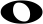
\includegraphics[scale=0.5]{img/whole_note}
}
&
\parbox{0.15\linewidth}{
\centering
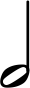
\includegraphics[scale=0.5]{img/half_note}
}
&
\parbox{0.15\linewidth}{
\centering
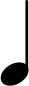
\includegraphics[scale=0.5]{img/quarter_note}
}
&
\parbox{0.15\linewidth}{
\centering
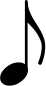
\includegraphics[scale=0.5]{img/eighth_note}
}
&
\parbox{0.15\linewidth}{
\centering
\includegraphics[scale=0.5]{img/meter}
}
\\
A whole note. & A half note. & A quarter note. & An eighth note & A 4/4 time signature\\

\end{tabular}
\end{table}

These durations are grouped together units called bars or measures. The time signature specifies how a bar is subdivided into metrical units. The time signature consists of two numbers written above each other as in table \ref{tab:notation}, when written in text we refer to this as a 4/4 time signature where the first number is the top number and the second number is the bottom number. The top number specifies the number of notes per measure, the bottom number specifies the units of those notes. The time signature is sometimes called meter.

Staff music notation is one of the most widespread representation of rhythmic structure. In field of rhythm analysis, another structure called a \textit{metrical grid} is popular. A metrical grid is a representation that contains several levels, where the lowest level corresponds to the smallest subdivided unit and the highest level corresponds to a bar. A metrical grid representing a 3/4 time signature is shown in figure \ref{fig:grid}. Bars are separated using a horizontal line, $\bullet$ symbols indicate the \textit{downbeats} of each level. The downbeats are the leftmost units metrical unit of a subdivided unit. Level three for example contains one downbeat per bar. Level three is subdivided into three level-two downbeats, the second and third of which is a level-three \textit{upbeat}. Every level-two unit is subdivided into two level-one downbeats, the second of which is a level-two upbeat. 

\begin{figure}
\centering
\hspace{2in}
\begin{tabular}{llllll|llllll|ll}
$\bullet$ &  &  &  &  &  & 		$\bullet$ &  &  &  &  &  & $\bullet$ & Level 3\\ 
$\bullet$ &  & 	$\bullet$ &  & 	$\bullet$ & & 	$\bullet$ & & $\bullet$ &  & $\bullet$ &  & $\bullet$ & Level 2\\
$\bullet$ & 		$\bullet$ & 		$\bullet$ & 		$\bullet$ & $\bullet$ & $\bullet$ & $\bullet$ & $\bullet$ & $\bullet$ & $\bullet$ & $\bullet$ & $\bullet$ & $\bullet$ & Level 1\\
\end{tabular}
\caption{Metrical grid of a 3/4 time signature.}
\label{fig:grid}
\end{figure}

Having now introduced two representations of rhythmic structure, we can turn to some the work done in this field.\cite{temperley2010modeling} studies the probabilistic properties of rhythmic structures in isolation. It is suggested that rhythm has some probabilistic characteristics that are shared to some extend by a wide range of musical styles. Temperley identifies a number of intuitions about rhythm that seem to be common-practice. These intuitions include the general tendency of onsets to fall on downbeats, the preference for onsets on upbeats to be preceded or followed by a note on the previous or next downbeat and the tendency of long notes to fall on downbeats. 

Temperley proposes six different models intended to be sensitive to these regularities. The adequacy of these models is evaluated by measuring their cross-entropy, using cross-validation on a corpus of European folk songs. Temperley's work shows that it is fairly easy to devise probabilistic models that differentiate common rhythms from less common rhythms. Intuitively, not every pattern of onsets that can by described as a valid rhythmic structure will be perceived as a rhythm by humans. 

% Metrical grids?

\section{Performances}
\label{sec:performances}

Rhythmic structure in itself does not imply onsets in absolute time. The common way to relate a rhythmic structure to a performance is by assigning some real duration to a metrical unit. The amount of real time we assign to a metrical duration is usually called the \textit{tempo}. Given a tempo, a rhythmic structure can be converted to a set of \textit{idealised} onset times, also called metronomic onset times. 

When humans perform a rhythm, they deviate from the idealised onset times in several ways. Unless a metronome is used, the tempo will usually fluctuate as the performance progresses. Much of this fluctuation is intentional and is referred to as \textit{musical expression}. Apart from global tempo changes humans deviate from idealised onsets locally as well, even when a metronome is used. Part of this deviation may be caused by imperfections in the performance and can be considered noise, another part can be the result of expression. In general, it is thought that a large proportion of deviation from idealised onsets is intentional and, of course depending on the competence of the performer, a small proportion of it is noise.

Although a performance deviates from the idealised onsets given by the structure and tempo, human listeners are often able to derive the rhythmic structure from a performance and multiple listeners tend to be quite consistent in their interpretations of a performance. 

Several authors have suggested models that try to mimic this human capacity. Several aspects of rhythmic structure have been studied separately: Beat-tracking systems simply try to track the tempo of a performance, not worrying about meter. In rhythm quantisation, every note of a performance is aligned to tries to estimate the length of a notes in a performance in terms of a beat. The structures produced by this sort of analysis still do not trivially show the time signature. Finally, meter-finding approaches try to derive the complete rhythmic structures from performances. Finding the complete rhythmic structure is essential for automatic music transcription, the production of musical scores, written in staff notation, based on performances.



In his book, \citet{temperley2007music} studies the probabilistic properties of rhythmic structures and proposes a system that if. 

Other authors that have been concerned with probabilistic models of rhythm have almost exclusively considered any form of expression to be noise. In a recent study, \citet{temperley2009unified} proposed a unified model of 

\section{An Expression-Aware Subdivision-Based Rhythmic Parser}
\label{sec:introducing}

% Therefore we present our expression model the way it is presented

% This approach is based on early work by longuet-higgins.
% We try to use regular expression to our advantage

Much of this expression appears to be a highly complicated and irregular process that is influenced by factors as musical style and the `mood' of the music, the audience and the performer. There is a field of research concerned with finding models for musical expression, see for example \citet{widmer2004computational}. Here, we will not concern ourselves with extensive models of expression. Instead, we will suggest that there may be more regular forms of local expression that are the result of a tendency of humans to emphasize downbeats.

This emphasis may materialise though performing downbeats slightly louder or stretching their duration slightly. 

We will evaluate our work on jazz performances but it should generalise to other music styles as well.